\chapter{Event detection and alerts}\label{ch:detect}

An observer cannot watch a screen all day. The purpose of an \emph{alert} is to say, without a human present, that
something happened: the ground moved more than it normally does. This chapter explains the standard way of
deciding that, the STA/LTA trigger \parencite{allen1978}, shows how it behaves on data whose true events are known,
and describes how RS3D's alert pipeline is designed around it.

\begin{rs3dwarn}[Status of this chapter]
Sections~\ref{sec:detprob} to~\ref{sec:failures} describe standard theory and measurements made with the
application's demo data and ObsPy's reference implementation. Section~\ref{sec:alertdesign} is a \emph{design proposal}: the alert feature
of RS3D is not yet implemented, and the proposal will be revised after it is.
\end{rs3dwarn}

\section{The detection problem}\label{sec:detprob}
Detection is a decision between two hypotheses at every instant: $H_0$, \emph{only background noise}, and $H_1$, \emph{noise
plus a seismic signal}. Any decision rule makes two kinds of mistakes: a \emph{false alarm} (declaring $H_1$ when $H_0$ is
true) and a \emph{missed detection} (declaring $H_0$ when $H_1$ is true). Lowering the threshold at which an event is
declared catches weaker events but raises the false-alarm rate, and vice versa; no rule escapes the trade-off, and the art
lies in choosing a rule whose false alarms are rare enough to tolerate at an acceptable sensitivity. For an alert that wakes
somebody at night the tolerable false-alarm rate is very low.

The difficulty is that seismic noise is not a fixed distribution. It changes with the time of day, the weather and the
neighbours' habits. A detector must therefore compare the \emph{present} signal with the \emph{recent} noise level,
not with a constant. This is the idea of the STA/LTA trigger.

\section{The characteristic function}\label{sec:cf}
Before averaging, the signal is turned into a non-negative \emph{characteristic function} (CF) $c[n]$ that grows when a signal is
present. The simplest choices are the squared amplitude, $c[n]=x[n]^{2}$ (an instantaneous power), or the absolute value
$\abs{x[n]}$. Allen's original function also includes the squared first difference, which responds to
abrupt changes. ObsPy's reference implementation, and RS3D's design, use $c[n]=x[n]^{2}$.

Two preprocessing steps are essential before the CF is formed.
\begin{enumerate}
\item \textbf{Remove the offset.} The DC component of raw counts (Chapter~\ref{ch:response}) would be squared into a huge
  constant that masks any event. A band-pass filter that rejects frequencies below the lower corner removes it.
\item \textbf{Band-pass filter, causally.} Restricting the signal to the band where the events of interest have their
  energy raises the signal-to-noise ratio. For the filter to be usable in real time and not to blur the onset
  (Chapter~\ref{ch:filter}) it must be \emph{causal}.
\end{enumerate}

\section{The classic STA/LTA}
Let $N_s$ and $N_l$ be the lengths, in samples, of a short and a long window, $N_s\ll N_l$. The short-term average (STA) and
long-term average (LTA) of the CF at sample $i$ are the means over the two \emph{trailing} windows:
\begin{equation}\label{eq:stalta}
  \mathrm{STA}_i = \frac{1}{N_s}\sum_{j=i-N_s+1}^{i} c[j],\qquad
  \mathrm{LTA}_i = \frac{1}{N_l}\sum_{j=i-N_l+1}^{i} c[j],\qquad
  R_i = \frac{\mathrm{STA}_i}{\mathrm{LTA}_i}.
\end{equation}
The STA follows the signal quickly and estimates the \emph{current} power; the LTA changes slowly and estimates the
\emph{background}. In quiet noise $R\approx1$. When an event arrives the STA rises almost at once while the LTA, which
averages over a long past, hardly moves, so $R$ jumps. The detector declares an event when $R$ crosses a
\emph{trigger-on threshold} $r_{\mathrm{on}}$ upward and ends it when $R$ falls below a lower \emph{trigger-off threshold}
$r_{\mathrm{off}}<r_{\mathrm{on}}$. Using two thresholds, \emph{hysteresis}, prevents rapid on--off flicker when $R$
hovers near one value.

\begin{figure}[tbp]
\centering
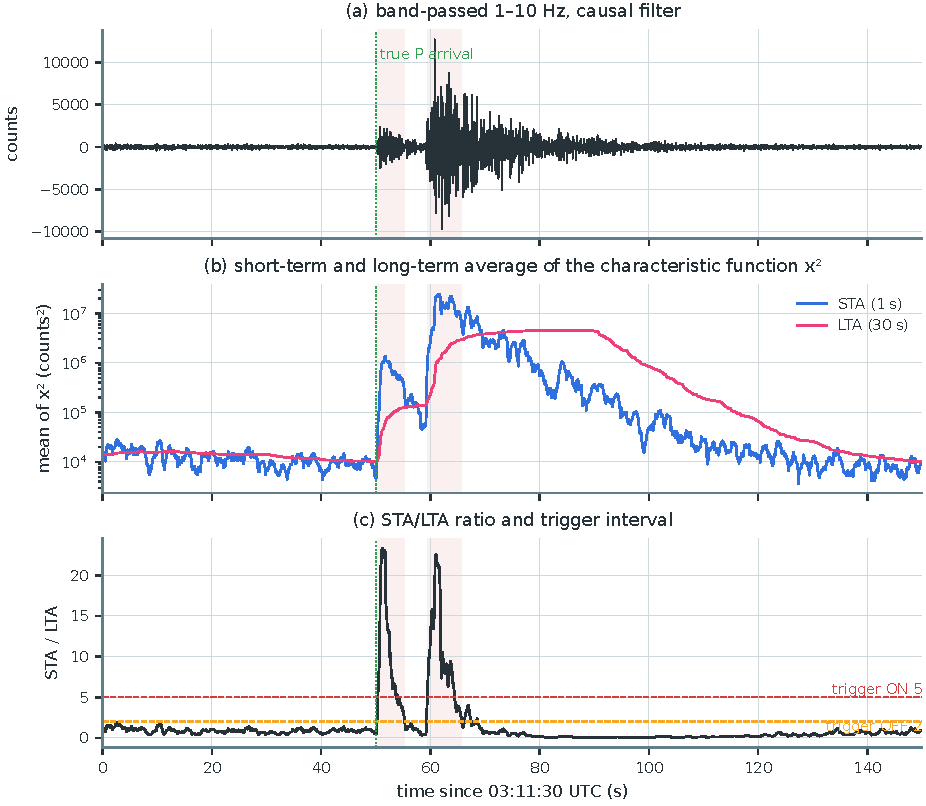
\includegraphics[width=\linewidth]{theory-stalta-example}
\caption{STA/LTA on the demo local earthquake (EHZ). (a) The signal band-passed 1--10~Hz with a causal filter. (b) STA (1~s)
and LTA (30~s) of the characteristic function $x^{2}$: the STA jumps by orders of magnitude at the P arrival while the LTA
lags. (c) The ratio, the thresholds ($r_{\mathrm{on}}=5$, $r_{\mathrm{off}}=2$) and the trigger intervals (pink). The ratio
falls back below the threshold between the P and the S wave, so the single earthquake produces two trigger intervals.}\label{fig:stalta}
\end{figure}

\subsection{The warm-up period}
$\mathrm{LTA}_i$ is meaningless until $N_l$ samples have been seen. ObsPy sets the ratio to zero for the first samples; a
live monitor must not raise an alert during this period, which is $N_l/\fs$ seconds long (30~s in the example).

\section{The recursive STA/LTA}
The classic form needs the last $N_l$ samples in memory. A \emph{recursive} variant replaces each moving average by an
exponential one:
\begin{equation}\label{eq:rec}
  \mathrm{STA}_i = \mathrm{STA}_{i-1} + \frac{c[i]-\mathrm{STA}_{i-1}}{N_s},\qquad
  \mathrm{LTA}_i = \mathrm{LTA}_{i-1} + \frac{c[i]-\mathrm{LTA}_{i-1}}{N_l}.
\end{equation}
Unrolling the recursion shows that sample $c[i-k]$ carries the weight $\frac1N(1-\frac1N)^k$: a geometric, not a
rectangular, window, with a \emph{time constant} of $N$ samples ($\tau_s=N_s/\fs$, $\tau_l=N_l/\fs$ seconds)
\parencite{withers1998,trnkoczy2012}. The recursion needs only two numbers of state and one multiplication per sample,
independent of $N_l$, which makes it the natural choice for a monitor that runs continuously on a stream.
For the same $N_s$ and $N_l$ the two forms give similar but not identical ratios.

\section{Setting the parameters}\label{sec:params}
The three groups of parameters have different roles; \textcite{trnkoczy2012} gives a systematic treatment.

\begin{description}[leftmargin=2.2cm,style=nextline]
\item[STA length] should be a few periods of the dominant signal frequency: long enough that the STA is not driven by a
  single large sample, short enough to react quickly. A short STA finds short, impulsive events; a long STA favours
  emergent ones. \Cref{fig:params} (left) shows the effect.
\item[LTA length] should be much longer than the STA (a factor of 10 or more) so that an event does not contaminate its own
  background estimate, yet short enough to follow the slow change of the noise. \Cref{fig:params} (right) shows the
  effect.
\item[Thresholds] $r_{\mathrm{on}}$ sets the sensitivity; $r_{\mathrm{off}}$, typically a fraction of $r_{\mathrm{on}}$, sets how
  long an event is held. The values of the example, $r_{\mathrm{on}}=5$ and $r_{\mathrm{off}}=2$, were chosen from the sweep of
  \cref{fig:sweep}.
\item[Pass band] the band in which the CF is formed; it should contain the energy of the target events and exclude
  the dominant noise.
\end{description}

\begin{figure}[tbp]
\centering
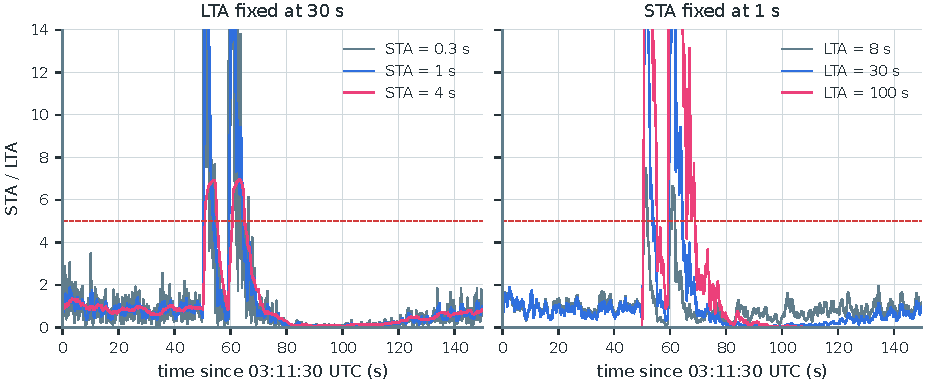
\includegraphics[width=\linewidth]{theory-stalta-params}
\caption{Effect of the window lengths on the ratio for the same earthquake. Left: STA of 0.3, 1 and 4~s with LTA 30~s. A
longer STA gives a lower, smoother peak. Right: LTA of 8, 30 and 100~s with STA 1~s. A short LTA is contaminated by the
event itself and the ratio collapses quickly. Dashed: threshold 5.}\label{fig:params}
\end{figure}

\subsection{Statistical meaning of the ratio}
If the signal is Gaussian noise and the CF is $x^{2}$, the average of $x^{2}$ over a window follows a scaled $\chi^{2}$
distribution. For noise that occupies a bandwidth $B$ (hertz) a window of $T$ seconds contains about $\nu\approx 2BT$
independent values, so STA and LTA have $\nu_s=2BT_s$ and $\nu_l=2BT_l$ degrees of freedom and, for stationary noise, the ratio $R$
follows an $F$ distribution with $(\nu_s,\nu_l)$ degrees of freedom. For the 1--10~Hz band ($B\approx9$~Hz) with a 1~s STA and a
30~s LTA this gives $\nu_s=18$ and $\nu_l=540$. The probability that a \emph{single} ratio value exceeds a threshold is then
tiny (\cref{tab:null}, second column): $1.4\times10^{-10}$ at $r=5$.

\begin{table}[tbp]
\centering\small
\caption{False alarms per day (events merged within 30~s) for stationary Gaussian noise and for the demo day, with the
$F$-distribution tail probability for one independent ratio value. Detector: causal 1--10~Hz band-pass, recursive STA/LTA,
STA 1~s, LTA 30~s, $r_{\mathrm{off}}=0.4\,r_{\mathrm{on}}$.}\label{tab:null}
\begin{tabular}{@{}rrrr@{}}
\toprule
Threshold & F tail $P(R>r)$ & Stationary noise & Demo day \\ \midrule
2 & 8.5e-03 & 89 & 498 \\
2.5 & 6.0e-04 & 0 & 240 \\
3 & 3.5e-05 & 0 & 83 \\
3.5 & 1.7e-06 & 0 & 25 \\
4 & 7.9e-08 & 0 & 7 \\
5 & 1.4e-10 & 0 & 0 \\
6 & 2.3e-13 & 0 & 0 \\
\bottomrule
\end{tabular}

\end{table}

The table's last two columns are the important result. For \emph{stationary} noise, false alarms disappear
above $r\approx 2.5$, as theory predicts. The demo day, whose noise changes with the time of day and fluctuates from
minute to minute, still produces 83 false events per day at $r=3$ and does not reach zero until $r=5$.
\emph{Real noise is not stationary}, the LTA lags behind every rise in the noise level, and a threshold chosen from
stationary theory is far too sensitive.

\begin{figure}[tbp]
\centering
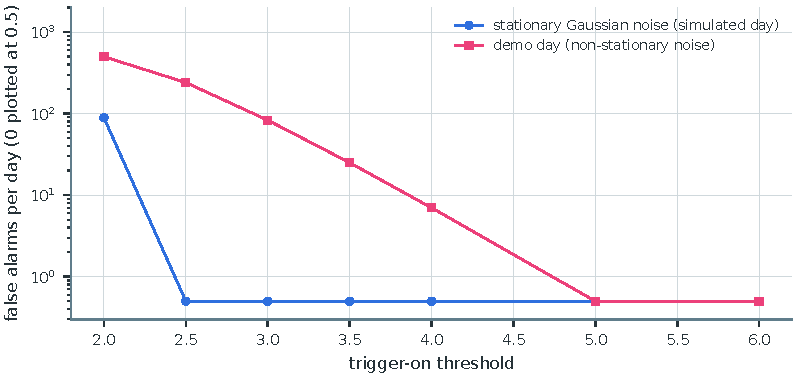
\includegraphics[width=\linewidth]{theory-stalta-null}
\caption{False alarms per day against threshold for stationary noise (blue) and the demo day (pink); zeros are plotted at
0.5 on the logarithmic axis.}\label{fig:null}
\end{figure}

\begin{rs3dkey}
The threshold must be chosen from the noise of \emph{your} site, over days, not from the theory of stationary noise.
A threshold that gives zero false alarms on stationary noise may give dozens per day on a real station.
\end{rs3dkey}

\section{Behaviour on the demo day}\label{sec:demoday}
\Cref{fig:staltaday} applies the detector (causal 1--10~Hz band-pass, recursive STA/LTA, STA 1~s, LTA 30~s,
$r_{\mathrm{on}}=5$, $r_{\mathrm{off}}=2$, events closer than 30~s merged) to the whole demo day. \Cref{tab:events}
lists the events found. All three are real in the sense that something happened; two of them are not earthquakes.

\begin{figure}[tbp]
\centering
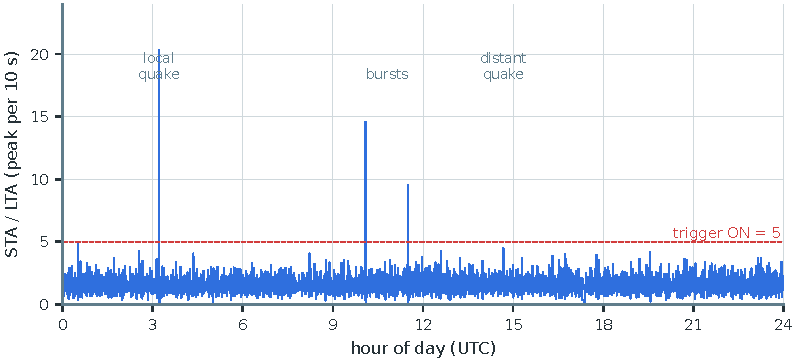
\includegraphics[width=\linewidth]{theory-stalta-day}
\caption{The STA/LTA ratio over the demo day (peak per 10~s). Three episodes cross the threshold of 5: the local earthquake
and the two noise bursts. The distant earthquake, whose energy is below 1~Hz, stays below it.}\label{fig:staltaday}
\end{figure}

\begin{table}[tbp]
\centering\small
\caption{Events detected on the demo day at $r_{\mathrm{on}}=5$. The ``cause'' is known because the demo data were constructed.}\label{tab:events}
\begin{tabular}{@{}lrrl@{}}
\toprule
Onset (UTC) & Duration (s) & Peak ratio & Cause \\ \midrule
03:12:20 & 18 & 20.3 & local earthquake \\
10:05:00 & 12 & 14.6 & noise burst \\
11:30:00 & 12 & 9.5 & noise burst \\
\bottomrule
\end{tabular}

\end{table}

\begin{figure}[tbp]
\centering
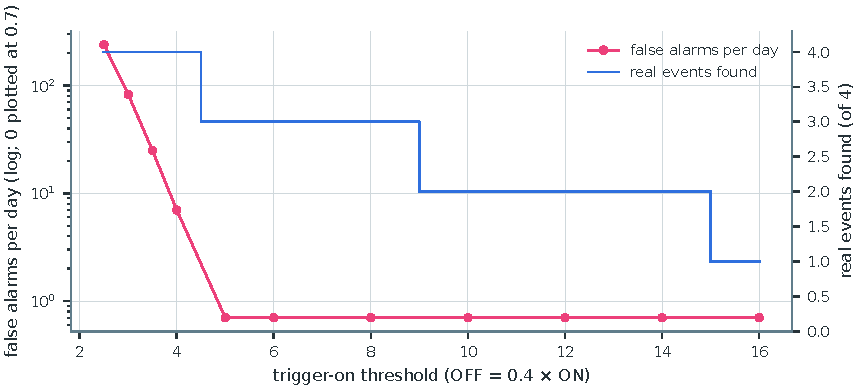
\includegraphics[width=\linewidth]{theory-stalta-sweep}
\caption{Sweep of the trigger-on threshold. False alarms (pink, left axis) vanish at 5; real events found (blue, right
axis) fall from 4 to 3 at that threshold, because the distant earthquake is lost, then to 2 and 1 as the two noise
bursts are lost one after the other; at the highest thresholds only the local earthquake remains.}\label{fig:sweep}
\end{figure}

\section{Failure modes and how to reduce them}\label{sec:failures}
\subsection{Man-made noise looks like an earthquake}
The two noise bursts of the demo day exceed the threshold by a wide margin: to an energy detector a person stamping next to
the sensor and a small local earthquake are both a sudden rise in power. \Cref{fig:compare} shows the difference that
can be exploited: the earthquake keeps a long, decaying \emph{coda} and the ratio stays elevated, whereas the
burst stops abruptly and the ratio collapses within seconds. Criteria that use this are a minimum duration, the ratio's
persistence, and the frequency content (the burst is broadband, the earthquake concentrated in 2--8~Hz).

\begin{figure}[tbp]
\centering
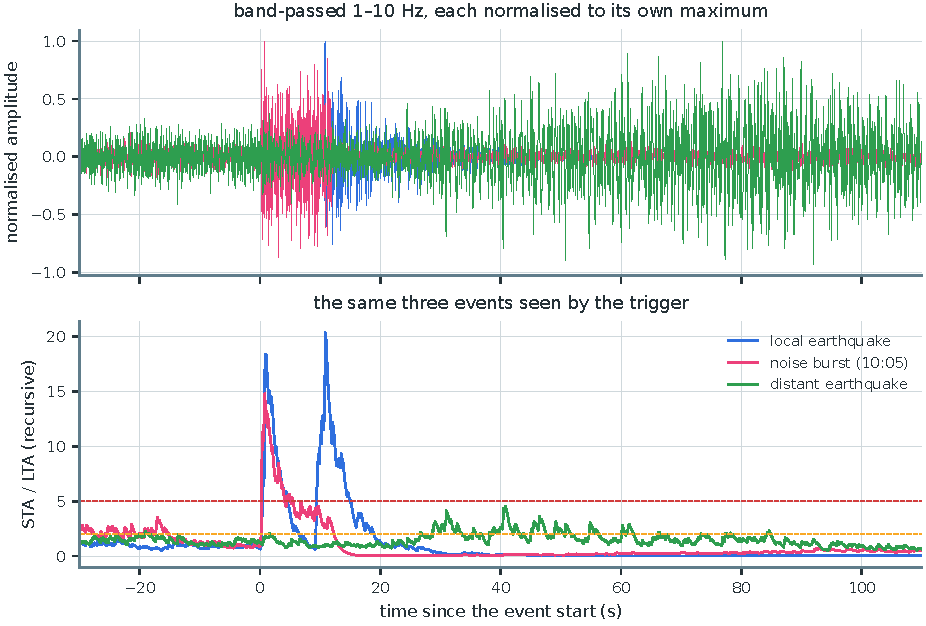
\includegraphics[width=\linewidth]{theory-stalta-compare}
\caption{Three events seen by the trigger, each aligned at its start. The earthquake (blue) keeps a decaying coda; the
burst (pink) stops after 12~s; the distant earthquake (green) never reaches the threshold because its energy lies
below the 1--10~Hz pass band.}\label{fig:compare}
\end{figure}

\subsection{Other failure modes}
\begin{description}[leftmargin=2.4cm,style=nextline]
\item[Gaps] a gap must reset the long average; otherwise the first samples after the gap are compared with a stale
  background. The detector treats each contiguous stretch separately and observes the warm-up period after each gap.
\item[Offset steps and spikes] a step in the DC level or a single instrument spike produces a short, large CF. The
  band-pass removes steps; a spike is removed by a minimum duration.
\item[LTA contamination] a long event raises the LTA and lowers the ratio for a while after it, so an aftershock may be
  missed. Some detectors \emph{freeze} the LTA while a trigger is active.
\item[Slow rise of noise] the LTA lags a steadily rising noise level, which keeps $R>1$; a rising wind can cause a
  false alarm.
\item[Weak distant events] emergent, long-period events lie outside a 1--10~Hz band; a detector for them needs a
  different band and longer windows (the sweep shows the distant earthquake lost already at $r=5$).
\end{description}

\section{Latency}\label{sec:latency}
How soon after an event begins does the trigger fire? Assume that the CF power jumps at $t=0$ from the background $P_0$ to
$P_1$ and that the LTA hardly changes in the first seconds. With the recursive STA of~\eqref{eq:rec}, whose time constant is
$\tau_s$,
\begin{equation}
  \mathrm{STA}(t) = P_1 + (P_0-P_1)\,e^{-t/\tau_s}.
\end{equation}
The ratio reaches $r_{\mathrm{on}}$ when $\mathrm{STA}=r_{\mathrm{on}}P_0$, at the delay
\begin{equation}\label{eq:delay}
  t_d = -\tau_s\,\ln\!\left(\frac{P_1-r_{\mathrm{on}}P_0}{P_1-P_0}\right),\qquad P_1>r_{\mathrm{on}}P_0 .
\end{equation}
Equation~\eqref{eq:delay} has two consequences. A strong event ($P_1\gg r_{\mathrm{on}}P_0$) triggers after a small fraction
of $\tau_s$: for a power increase of $100\times$ and $r_{\mathrm{on}}=5$, $t_d=0.04\,\tau_s$. A weak event
($P_1\to r_{\mathrm{on}}P_0$) takes arbitrarily long, and one with $P_1\le r_{\mathrm{on}}P_0$ is never detected at all.
(Appendix~\ref{app:delay} derives the formula.) The trigger time is therefore a \emph{detection} time, not an onset
time; for the onset the pass band must be causal and a dedicated picker must refine it.

\section{Design of the RS3D alert pipeline}\label{sec:alertdesign}
\begin{rs3dwarn}[Design proposal]
The following is the design that is planned for the first implementation. It will be revised when the feature is built.
\end{rs3dwarn}

\paragraph{Goals.} Detect events on the live stream without a browser open; tell the user through the channels they
enabled; keep a permanent record; and never fail silently.

\paragraph{Architecture.} The detector runs as a background service inside the application process, fed from the same
ring buffer as the Live page (Chapter~\ref{ch:realtime}), so it keeps running when no browser tab is open.
\Cref{fig:alertarch} shows the stages and \cref{fig:alertstate} the logic of one detector.

\begin{figure}[tbp]
\centering
\resizebox{\linewidth}{!}{\begin{tikzpicture}[node distance=5mm and 8mm]
  \node[box] (buf) {ring buffer\\[-1pt]{\scriptsize live samples}};
  \node[box,right=of buf] (pre) {pre-processing\\[-1pt]{\scriptsize causal band-pass}};
  \node[box,right=of pre] (det) {STA/LTA\\[-1pt]{\scriptsize recursive}};
  \node[boxblue,right=of det] (logic) {event logic\\[-1pt]{\scriptsize thresholds, hold-off}};
  \node[box,below=of logic,xshift=-18mm] (s1) {on-screen\\[-1pt]{\scriptsize banner, sound}};
  \node[box,right=of s1] (s2) {desktop\\[-1pt]{\scriptsize notification}};
  \node[box,right=of s2] (s3) {message\\[-1pt]{\scriptsize Telegram, e-mail}};
  \node[box,right=of s3] (s4) {record\\[-1pt]{\scriptsize plot and log}};
  \draw[flow] (buf) -- (pre); \draw[flow] (pre) -- (det); \draw[flow] (det) -- (logic);
  \foreach \s in {s1,s2,s3,s4} {\draw[flow] (logic.south) -- ++(0,-2mm) -| (\s.north);}
\end{tikzpicture}}
\caption{Proposed alert pipeline. Each output on the bottom row is an independent switch in Settings, and the record is
always written.}\label{fig:alertarch}
\end{figure}

\begin{figure}[tbp]
\centering
\begin{tikzpicture}[node distance=14mm,every node/.style={font=\small\sffamily}]
  \node[boxdark] (warm) {warm-up};
  \node[boxblue,right=18mm of warm] (idle) {idle};
  \node[box,right=24mm of idle,fill=rs3dred!15,draw=rs3dred] (act) {active};
  \node[box,right=18mm of act] (cool) {hold-off};
  \draw[flow] (warm) -- node[above]{$N_l$ samples} (idle);
  \draw[flow] (idle) -- node[above]{$R>r_{\mathrm{on}}$} (act);
  \draw[flow] (act) -- node[above]{$R<r_{\mathrm{off}}$} (cool);
  \draw[flow] (cool.south) -- ++(0,-8mm) -| node[pos=0.25,below]{quiet for hold-off} (idle.south);
  \draw[flow] (cool.north) -- ++(0,6mm) -| node[pos=0.25,above]{$R>r_{\mathrm{on}}$ again: same event} (act.north);
  \draw[flow,dashed] (idle.north) -- ++(0,9mm) -| node[pos=0.25,above]{gap: restart} (warm.north);
\end{tikzpicture}
\caption{State of one detector. A new crossing during the hold-off period extends the same event, which is how the two
trigger intervals of \cref{fig:stalta} become one event.}\label{fig:alertstate}
\end{figure}

\paragraph{Event record.} Each event stores the onset time, the duration, the peak STA/LTA ratio, the peak amplitude (in counts, and in
m/s if the response is cached), the dominant frequency, the channel(s), and a snapshot of the waveform with its helicorder
position. This is what the user sees in the notification and what the saved plot and log contain.

\paragraph{Proposed initial parameters.} They come from the demo-day analysis above and are meant as a starting point to be
tuned on real data from the user's site.

\begin{table}[tbp]
\centering\small
\caption{Proposed initial alert parameters (design proposal).}\label{tab:alertparams}
\begin{tabularx}{\linewidth}{@{}l c X@{}}
\toprule
Parameter & Initial value & Reason\\ \midrule
Channel & EHZ & the vertical channel carries the P wave cleanly\\
Band-pass & 1--10~Hz, causal 4th order & local events; matches the Live default\\
STA / LTA & 1~s / 30~s & \cref{fig:stalta,fig:params}\\
$r_{\mathrm{on}}$ / $r_{\mathrm{off}}$ & 5 / 2 & zero false alarms on the demo day (\cref{fig:sweep})\\
Hold-off & 30 s & merges the P and S trigger intervals\\
Minimum duration & 2 s & rejects single-sample spikes\\
Warm-up & $N_l/\fs$ and after every gap & the LTA is not valid before\\
\bottomrule
\end{tabularx}
\end{table}

\paragraph{Known limitation.} An energy trigger cannot tell an earthquake from a burst of equal power. The first release will
report both, label an event ``short, no coda'' when it ends within a few seconds, and leave the decision to the user. The
criteria of Section~\ref{sec:failures} are candidates for later versions.

\paragraph{Comparison with rsudp.} The widely used \emph{rsudp} software \parencite{rsudp} also raises alerts from an
STA/LTA ratio on a Raspberry Shake stream. Community examples use a 6~s STA and a 30~s LTA and thresholds between about 1 and
4, with the observation that suitable thresholds depend strongly on the filter band and on site noise; no authoritative list of
its built-in defaults could be located while this manual was written, so none is quoted here. RS3D's alerts are intended to
complement it, with the added record-keeping and the helicorder and detail views of the application.
